For starting calculations, we will consider the mass of our payload at 100g. Then, the total mass of the rocket is 451g ($ p = \frac{m_p}{m_0} = 0.21 $). For the choice of the engine we used the formula $ T = k \cdot m_0 \cdot g_0 $ , which gives us that the average thrust is between 44.49N and 53.39N. Thus, we chose 2 D9-5 engines.

Depending on the materials, their densities, properties, and roles in 2.2.4. , using the program OpenRocket, we got these next parameters:
\begin{itemize}
    \item Length of 380 mm, Diameter of 50 mm, Total Mass 466g, Utile Mass 100g (p=21.45\%); 
    \item Stability coefficient 1.66 ; CG 18.4cm ; CP 26.7 cm; 
    \item Apogee 256m, max velocity 64.3 $ \frac{m}{s} $, max acceleration 96.6 $ \frac{m}{s^2} $, optimum delay of 5.84s, flight time 44.4s, ground hit velocity 7.07 $ \frac{m}{s} $;
    \item After the simulations, we concluded that the optimum diameter of the parachute for the payload is 217 mm and for the rocket body and cone 417 mm.
\end{itemize}

\begin{multicols}{2}

\begin{figure}[H]
\centering
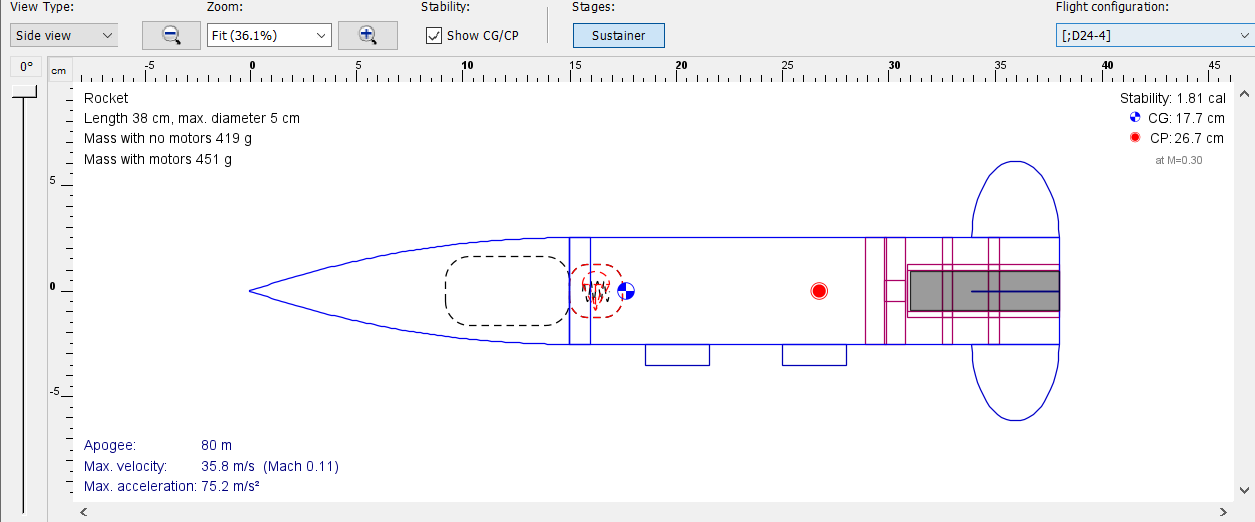
\includegraphics[width=0.7\linewidth]{side_view}
\caption{Side view and details from OpenRocket}
\end{figure}

\begin{figure}[H]
\centering
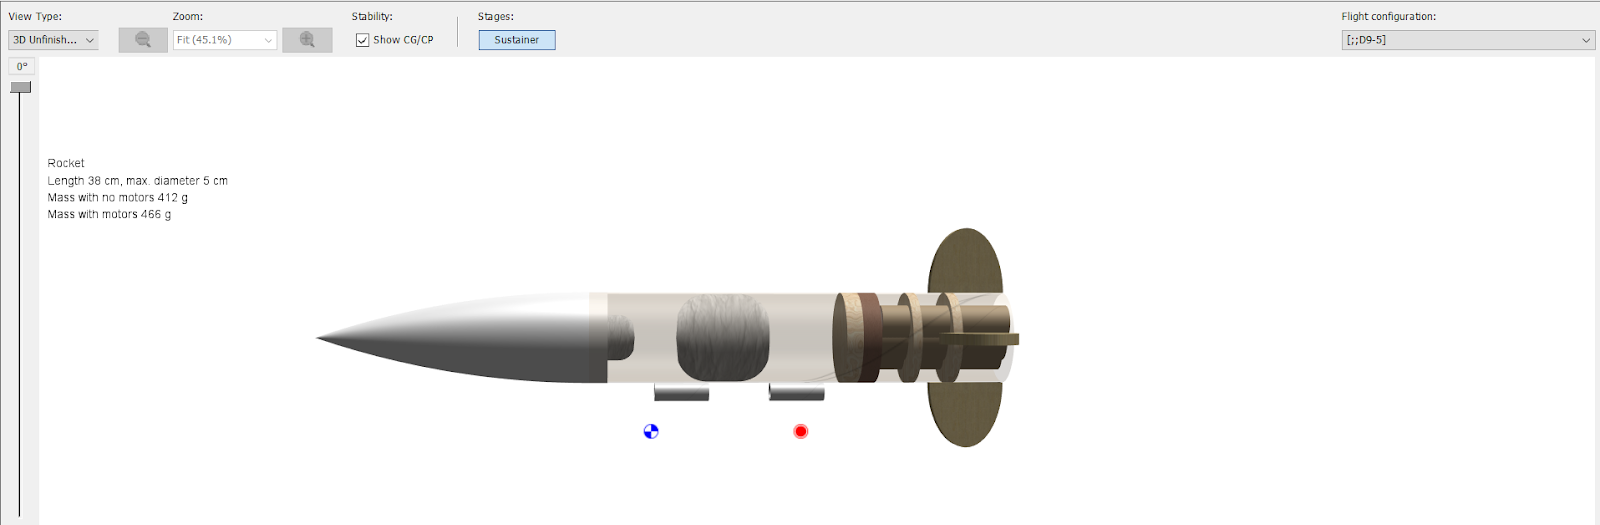
\includegraphics[width=0.8\linewidth]{unfinished_view}
\caption{3D Unfinished view}
\end{figure}

\begin{figure}[H]
\centering
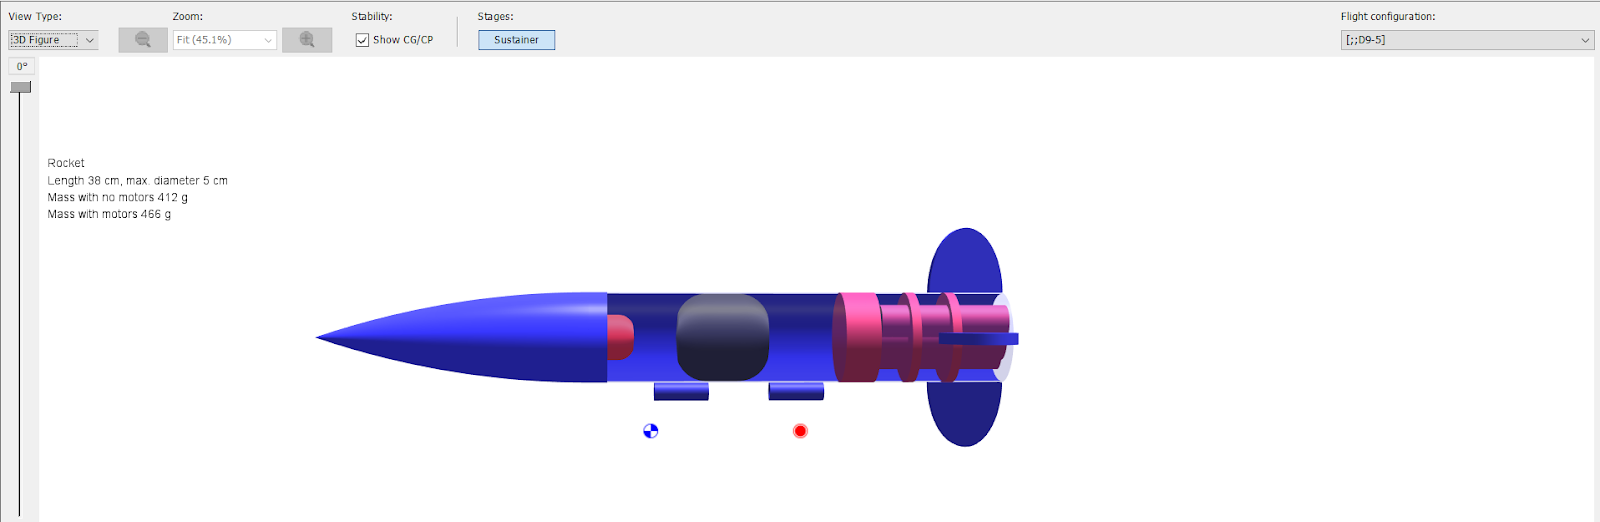
\includegraphics[width=0.8\linewidth]{figure}
\caption{3D Figure}
\end{figure}

\begin{figure}[H]
\centering
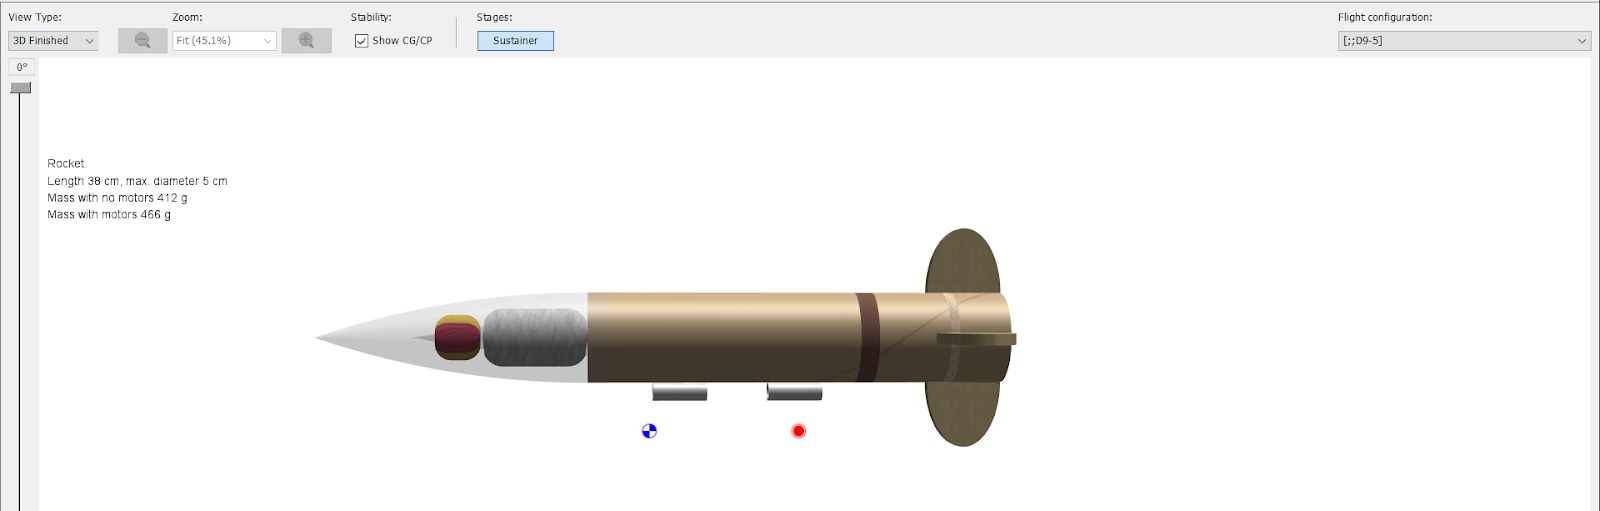
\includegraphics[width=0.8\linewidth]{finished_view}
\caption{3D Finished view}
\end{figure}

\end{multicols}

\begin{figure}[H]
\centering
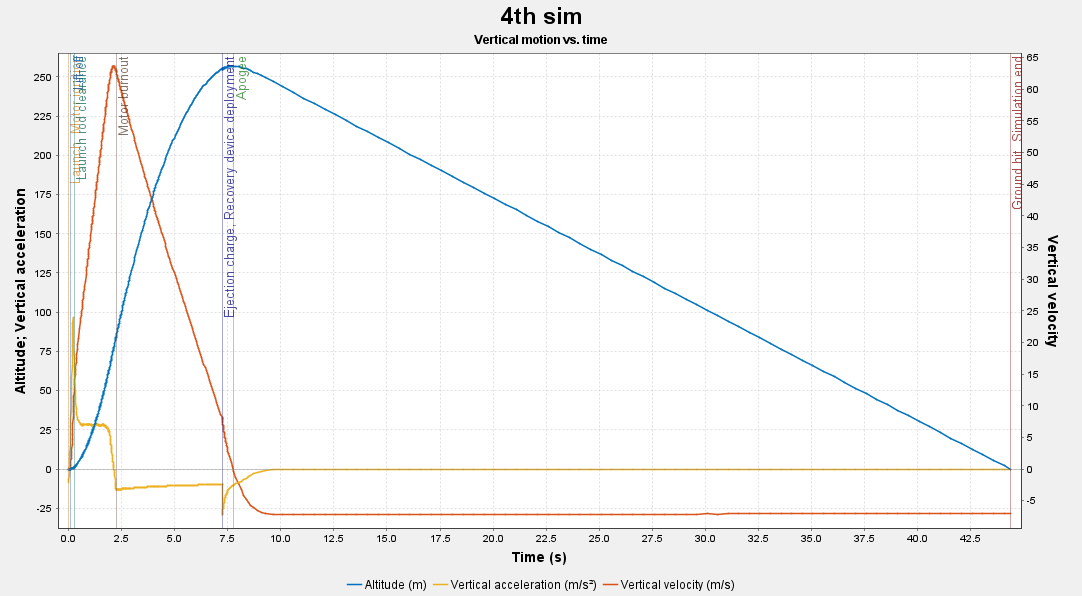
\includegraphics[width=0.8\linewidth]{graph}
\caption{Flight graph}
\end{figure}

\begin{figure}[H]
\centering
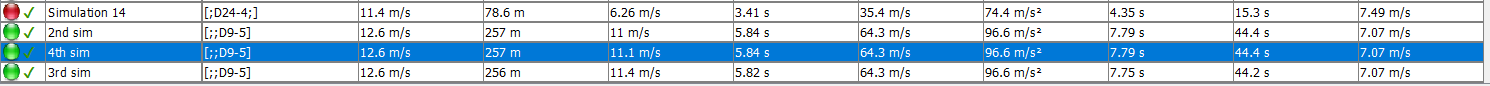
\includegraphics[width=0.9\linewidth]{simulation}
\caption{Simulation results}
\end{figure}

Calculation of the diameters of the parachutes:

$ \sqrt{\frac{2 \cdot 9.81 \cdot 0.1}{1.225 \cdot 0.8 \cdot 7.34^2} \cdot \frac{4}{3.14}} \cdot 1000 = 217.573 \mathrm{mm} $

$ \sqrt{\frac{2 \cdot 9.81 \cdot 0.369}{1.225 \cdot 0.8 \cdot 7.34^2} \cdot \frac{4}{3.14}} \cdot 1000 = 417.944 \mathrm{mm} $

